\documentclass[xcolor={dvipsnames},aspectratio=169,10pt]{beamer}
\usetheme{mx}
\usepackage{graphicx}
\graphicspath{{figures/}}
%% utility packages
\usepackage{etoolbox}
\usepackage{multicol}
\usepackage{relsize}
\usepackage{fontawesome}

% better text justifying
\usepackage{microtype}
% justify text inside list environment
% Ref: http://liam0205.me/2017/04/11/justifying-in-beamer-s-lists/
\usepackage{ragged2e}
\makeatletter
\patchcmd{\itemize}{\raggedright}{\justifying}{}{}
\patchcmd{\beamer@enum@}{\raggedright}{\justifying}{}{}
\patchcmd{\@@description}{\raggedright}{\justifying}{}{}
\makeatother

% table of content with numbers and justification
% https://tex.stackexchange.com/questions/188773
\setbeamertemplate{section in toc}{\hspace*{1em}\inserttocsectionnumber.~\inserttocsection\par}
\setbeamertemplate{subsection in toc}{\hspace*{2em}\inserttocsectionnumber.\inserttocsubsectionnumber.~\inserttocsubsection\par}

% math related packages
\usepackage{amsmath}
\usepackage[ruled,vlined]{algorithm2e}
\SetAlCapNameFnt{\scriptsize}
\SetAlCapFnt{\scriptsize}
\SetAlFnt{\scriptsize}

% figure related packages
\usepackage{graphicx}
\usepackage[scale=2]{ccicons}
\usepackage{qrcode}
\usepackage{tikz}
\usepackage{tikzpagenodes}
\usetikzlibrary{positioning}

% table related packages
\usepackage{array}
\usepackage{booktabs}
\usepackage{multirow}
\usepackage{colortbl}
\newcommand{\tabincell}[2]{\begin{tabular}{@{}#1@{}}#2\end{tabular}}

% code highlight
\usepackage{listings}
%\usepackage{minted}
%\definecolor{mintedbg}{HTML}{E5E9F0}
%\setminted{autogobble,bgcolor=mintedbg,fontsize=\small}
%\setmintedinline{bgcolor=mintedbg,fontsize=\smaller}
%\newminted{bash}{}
%\newminted{latex}{}
%\newmintinline{bash}{}
%\newmintinline{latex}{}
%\newcommand{\texdoc}[2]{\href{#2}{\bashinline|texdoc #1|}}

% hyperref setting
\hypersetup{
  unicode,
  psdextra,
  bookmarksnumbered=true,
  bookmarksopen=true,
  bookmarksopenlevel=3,
  bookmarksdepth=4,
  pdfcenterwindow=true,
  pdfstartview={Fit},
  pdfpagemode={FullScreen},
  pdfpagelayout={SinglePage},
}
\usepackage{bookmark}

% beamer theme
\usetheme{metropolis}
\metroset{block=fill,numbering=fraction}

% caption style
\usepackage{subcaption}
\setlength\abovecaptionskip{3pt}
\setbeamerfont{caption}{size=\scriptsize}
\renewcommand{\figurename}{Fig.}
\captionsetup{labelformat=empty,labelsep=none,textfont={bf,it}}

% Ref: https://github.com/gpoore/minted/blob/master/source/minted.dtx
\newenvironment{latexexample}
{\VerbatimEnvironment\begin{VerbatimOut}[gobble=3]{example.out}}{\end{VerbatimOut}%
  \begin{center}
    \begin{minipage}{0.47\linewidth}%
      \inputminted[resetmargins,fontsize=\scriptsize]{latex}{example.out}%
    \end{minipage}%
    \hspace{0.05\linewidth}%
    \begin{minipage}{0.47\linewidth}%
      \begin{framed}
        \setlength{\parindent}{2em}%
        \input{example.out}%
      \end{framed}
    \end{minipage}%
  \end{center}
}

\newenvironment{mathexample}
{\VerbatimEnvironment\begin{VerbatimOut}[gobble=3]{example.out}}{\end{VerbatimOut}%
  \begin{center}
    \begin{minipage}{0.47\linewidth}%
      \inputminted[resetmargins,fontsize=\scriptsize]{latex}{example.out}%
    \end{minipage}%
    \hspace{0.05\linewidth}%
    \begin{minipage}{0.47\linewidth}%
      \begin{framed}
        \[ \input{example.out} \]
      \end{framed}
    \end{minipage}%
  \end{center}
}

\newenvironment{mathexamples}
{\VerbatimEnvironment\begin{VerbatimOut}[gobble=3]{example.out}}{\end{VerbatimOut}%
  \begin{center}
    \begin{minipage}{0.47\linewidth}%
      \inputminted[resetmargins,fontsize=\scriptsize]{latex}{example.out}%
    \end{minipage}%
    \hspace{0.05\linewidth}%
    \begin{minipage}{0.47\linewidth}%
      \begin{framed}
        \directlua{
          local first = true
          for line in io.lines('example.out') do
          if first then
          first = false
          else
          tex.print('\\newline ')
          end
          tex.print('$' .. line .. '$')
          end
        }
      \end{framed}
    \end{minipage}%
  \end{center}
}



%---------------------------------------------------------------------
% Add Paper using {\paper{}. begin{beawer} ... end{beamer} }
%---------------------------------------------------------------------
\newcommand\paper[1]{
	\setbeamertemplate{footline}
	{
		\begin{beamercolorbox}[wd=\textwidth,ht=3mm,dp=03mm,leftskip=0.3cm,rightskip=0.3cm]{black}%
        		\usebeamerfont{page number in head/foot}
			(#1)\mbox{}\hfill\insertframenumber
		\end{beamercolorbox}%
	}
}


\title{  
%Prototyping Good AL/ML practices for Medical Image Synthesis
Good practices in AI/ML for Medical Image Synthesis %Fri 19 May 11:54:10 BST 2023
} 
\subtitle{
The deep learning and computer vision Journal club \\
UCL Centre for Advance Research Computing
}

\author{
Harvey Mannering, Sofia Mi\~nano, and  \\ 
{\bf Miguel Xochicale} (\faTwitter @\_mxochicale  \faGithub @mxochicale)
}
\date{
1st of June 2023
%\today
}
\institute{
Advanced Research Computing Centre and WEISS at University College London 
}

\githubrepository{https://github.com/mxochicale/medisynth}
\begin{document}
\maketitle

\begin{frame}
\frametitle{Table of Contents}
    \tableofcontents
\end{frame}


\section{Medical Image Synthesis}
\subsection{Background}
\begin{frame}
  \frametitle{Table of Contents}
  \tableofcontents[currentsection]
\end{frame}



%%%%%%%%%%%%%%%%%%%%%%%%%%%%%%%%%%%%%%%%%%%%%%%%%%%%%%%%
{
\paper{
Yi X., Walia E., and Babyn P., "Generative adversarial network in medical imaging: A review." Medical image analysis 58 (2019): 101552.
}

\begin{frame}{Generative adversarial network in medical imaging}{}
      \begin{figure}
        \centering
        \includegraphics[width=1.0\textwidth]{gans-in-medimg-applications/outputs/drawing-v00}
        % \caption{The sonographer-probe-patient control system}
      \end{figure}
\end{frame}
}

%%%%%%%%%%%%%%%%%%%%%%%%%%%%%%%%%%%%%%%%%%%%%%%%%%%%%%%%
{
\paper{
Yi X., Walia E., and Babyn P., "Generative adversarial network in medical imaging: A review." Medical image analysis 58 (2019): 101552.
}

\begin{frame}{Generative adversarial network in medical imaging}{}
      \begin{figure}
        \centering
        \includegraphics[width=1.0\textwidth]{gans-in-medimg-task-modalities-papers/outputs/drawing-v00}
        % \caption{The sonographer-probe-patient control system}
      \end{figure}
\end{frame}
}




\subsection{Methods}

%%%%%%%%%%%%%%%%%%%%%%%%%%%%%%%%%%%%%%%%%%%%%%%%%%%%%%%%
{
\paper{
Yi X., Walia E., and Babyn P., "Generative adversarial network in medical imaging: A review." Medical image analysis 58 (2019): 101552.
}

\begin{frame}{GANs background}
% \BigSizeFont
\begin{itemize}

\item Challenges in optimisitation
    \begin{itemize}
    \item Balance and stabilisation for training of $G$ and $D$, 
    \item Mode collapse (limiting learning to few modes)
    \end{itemize}

\item Varians of GANS
    \begin{itemize}
    \item Varying objective of $D$
    \item Varying objective of $G$
    \item Varying arquitecture
    \end{itemize}

\end{itemize}

\end{frame}
}



%%%%%%%%%%%%%%%%%%%%%%%%%%%%%%%%%%%%%%%%%%%%%%%%%%%%%%%%
{
\paper{
Yi X., Walia E., and Babyn P., "Generative adversarial network in medical imaging: A review." Medical image analysis 58 (2019): 101552.
}

\begin{frame}{Generative adversarial network in medical imaging}{}
      \begin{figure}
        \centering
        \includegraphics[width=1.0\textwidth]{gans-in-medimg-variants/outputs/drawing-v00}
        % \caption{The sonographer-probe-patient control system}
      \end{figure}
\end{frame}
}






\subsection{Applications}


\section{Good practices in AI/ML and checklists}
\begin{frame}
  \frametitle{Table of Contents}
  \tableofcontents[currentsection]
\end{frame}

%\subsection{checklist for artificial intelligence in medical imaging (CLAIM)}

\subsection{FDA-approved AI-based Medical Devices}

%%%%%%%%%%%%%%%%%%%%%%%%%%%%%%%%%%%%%%%%%%%%%%%%%%%%%%%%
{
\paper{
Benjamens S., Dhunnoo  P. and  Mesk\'o B. The state of artificial intelligence-based FDA-approved medical devices and algorithms: an online database. npj Digit. Med. 3, 118 (2020).
}
\begin{frame}{
FDA-approved AI-based Medical Devices
}{
%(2019-2021) @ KCL
}
      \begin{figure}
        \centering
        \includegraphics[width=1.0\textwidth]{fda-approved-ai-based-med-devs/outputs/drawing-v00}
        % \caption{The sonographer-probe-patient control system}
      \end{figure}
\end{frame}
}


\subsection{Quality Systems and Good Machine Learning Practices (GMLP) by FDA}
%%%%%%%%%%%%%%%%%%%%%%%%%%%%%%%%%%%%%%%%%%%%%%%%%%%%%%%%
{
\paper{
%\url{https://www.fda.gov/files/medical%20devices/published/US-FDA-Artificial-Intelligence-and-Machine-Learning-Discussion-Paper.pdf}
US-FDA-Artificial-Intelligence-and-Machine-Learning-Discussion-Paper
}
\begin{frame}{
Regulatory Framework for Modifications to \\
(AI/ML)-Based Software as a Medical Device (SaMD)
}{
%(2019-2021) @ KCL
}
      \begin{figure}
        \centering
        \includegraphics[width=1.0\textwidth]{goodALMLFDA/outputs/drawing-v00}
        % \caption{The sonographer-probe-patient control system}
      \end{figure}
\end{frame}
}




\section{Ultrasound Fetal Brain Images}

%%%%%%%%%%%%%%%%%%%%%%%%%%%%%%%%%%%%%%%%%%%%
\subsection{Clinical background and research aims}
\begin{frame}
  \frametitle{Table of Contents}
  \tableofcontents[currentsection]
\end{frame}


%%%%%%%%%%%%%%%%%%%%%%%%%%%%%%%%%%%%%%%%%%%%%%%%%%%%%%%%
{
\paper{
Wright-Gilbertson M. 2014 in PhD thesis; \url{https://en.wikipedia.org/wiki/Gestational_age}; 
National-Health-Service 2021. Screening for down’s syndrome, edwards’ syndrome and patau’s syndrome. \url{https://www.nhs.uk/pregnancy/your-pregnancy-care} 
}

\begin{frame}{Dating US scan (12-week scan)}{Clinical background}
      \begin{figure}
        \centering
        \includegraphics[width=1.0\textwidth]{dating-us-scan-12-week-scan/outputs/drawing-v02}
        % \caption{The sonographer-probe-patient control system}
      \end{figure}
\end{frame}
}



%%%%%%%%%%%%%%%%%%%%%%%%%%%%%%%%%%%%%%%%%%%%%%%%%%%%%%%%
{
\paper{
Sciortino et al. in Computers in Biology and Medicine 2017 https://doi.org/10.1016/j.compbiomed.2017.01.008; 
He et al. in Front. Med. 2021 https://doi.org/10.3389/fmed.2021.729978
Thomas L. A. van den Heuvel et al. https://hc18.grand-challenge.org/
Burgos-Artizzu, X et al. (2020). FETAL PLANES DB: Common maternal-fetal ultrasound images [Data set]. In Nature Scientific Reports (1.0, Vol. 10, p. 10200). Zenodo. https://doi.org/10.5281/zenodo.3904280
}
\begin{frame}{Challenges in Ultrasound biometric measurements}{Clinical background}

\begin{itemize}
% \item Operator dependant
% \item Position of the fetus
% \item Similar morphological and echogenic characteristics in the US image
% \item Threshold selection of the binary masks 
% \item Few public datasets are available [Thomas et. al 2018; Burgos-Artizzu et al. 2010]
%https://www.nature.com/articles/jhg200888
\item intra-view variability of imaging equipment and inter-observer variability of sonographer skills,
\item availability of expert clinicians or trained technicians to collect, to select, to classify and to validate regions of interest,
\item the cost of acquisition of clinical data as it requires expensive imaging equipment and experts for data collection and validation
\item the insufficient and limited amount of clinical data,
\item data accessibility due to patient privacy or protection of personal health information,
\end{itemize}

\end{frame}
}



%\section{Research aims}
%\begin{frame}
%  \frametitle{Table of Contents}
%  \tableofcontents[currentsection]
%\end{frame}



%%%%%%%%%%%%%%%%%%%%%%%%%%%%%%%%%%%%%%%%%%%%%%%%%%%%%%%%
{
%\paper{Wright-Gilbertson M. 2014 in PhD thesis}
\begin{frame}{Research aims}

\bigSizeFont
\begin{itemize}
\item Investigate and implement GAN-based and Diffusion-based models to synthetise realistic high-quality fetal ultrasound images
% of three fetal planes: trans-thalamic; trans-ventricular and trans-cerebellum.
% \item Propose and apply methods to evaluate quantitative and qualitative images of abnormal cases [High-risk]
\end{itemize}

\end{frame}
}


\subsection{Datasets of Fetal Brain Ultrasound Images}
\begin{frame}
  \frametitle{Table of Contents}
  \tableofcontents[currentsection]
\end{frame}


%%%%%%%%%%%%%%%%%%%%%%%%%%%%%%%%%%%%%%%%%%%%%%%%%%%%%%%%
{
\paper{
Burgos-Artizzu, X et al. (2020). FETAL PLANES DB: Common maternal-fetal ultrasound images [Data set]. In Nature Scientific Reports (1.0, Vol. 10, p. 10200). Zenodo. https://doi.org/10.5281/zenodo.3904280
}

\begin{frame}{TransThalamic}{Datasets of Fetal Brain Ultrasound Images}
      \begin{figure}
        \centering
        \includegraphics[width=1.0\textwidth]{fetal-planes-dataset-TransThalamic/outputs/drawing-v00}
        %\caption{}
      \end{figure}
\end{frame}
}

%%%%%%%%%%%%%%%%%%%%%%%%%%%%%%%%%%%%%%%%%%%%%%%%%%%%%%%%
{
\paper{
Burgos-Artizzu, X et al. (2020). FETAL PLANES DB: Common maternal-fetal ultrasound images [Data set]. In Nature Scientific Reports (1.0, Vol. 10, p. 10200). Zenodo. https://doi.org/10.5281/zenodo.3904280
}

\begin{frame}{TransCerebellum Plain}{Datasets of Fetal Brain Ultrasound Images}
      \begin{figure}
        \centering
        \includegraphics[width=1.0\textwidth]{fetal-planes-dataset-TransCerebellum/outputs/drawing-v00}
        %\caption{}
      \end{figure}
\end{frame}
}





%%%%%%%%%%%%%%%%%%%%%%%%%%%%%%%%%%%%%%%%%%%%%%%%%%%%%%%%
{
\paper{
Burgos-Artizzu, X et al. (2020). FETAL PLANES DB: Common maternal-fetal ultrasound images [Data set]. In Nature Scientific Reports (1.0, Vol. 10, p. 10200). Zenodo. https://doi.org/10.5281/zenodo.3904280
}

\begin{frame}{TransVentricular Plane}{Datasets of Fetal Brain Ultrasound Images}
      \begin{figure}
        \centering
        \includegraphics[width=1.0\textwidth]{fetal-planes-dataset-TransVentricular/outputs/drawing-v00}
        %\caption{}
      \end{figure}
\end{frame}
}






\subsection{Machine Learning Pipeline}
\begin{frame}
  \frametitle{Table of Contents}
  \tableofcontents[currentsection]
\end{frame}

%%%%%%%%%%%%%%%%%%%%%%%%%%%%%%%%%%%%%%%%%%%%%%%%%%%%%%%%
{
% \paper{Private github repository: \url{https://github.com/xfetus/synthetic-foetuses​ }}
\begin{frame}{Machine Learning Pipeline}{Fetal US imaging synthesis with GANs}
      \begin{figure}
        \centering
        \includegraphics[width=1.0\textwidth]{machine-learning-pipeline/outputs/drawing-v01}
        %\caption{}
      \end{figure}
\end{frame}
}



\subsection{Methods}
\begin{frame}
  \frametitle{Table of Contents}
  \tableofcontents[currentsection]
\end{frame}


%%%%%%%%%%%%%%%%%%%%%%%%%%%%%%%%%%%%%%%%%%%%%%%%%%%%%%%%
{
\paper{
M. Iskandar et al.  "Towards Realistic Ultrasound Fetal Brain Imaging Synthesis" in MIDL2023
\faGithub \, \url{https://github.com/budai4medtech/midl2023}
}
\begin{frame}{Image Quality Assessment}{Methods}
      \begin{figure}
        \centering
        \includegraphics[width=1.0\textwidth]{Image-Quality-Assessment/outputs/drawing-v00}
%         \caption{(a) DCGAN arquitecture, loss functions for DC-GANs and batches of synthetic fetal head images,
% 		(b) FASTGAN arquitecture and batches of synthethic fetal head images}
      \end{figure}
\end{frame}
}



%%%%%%%%%%%%%%%%%%%%%%%%%%%%%%%%%%%%%%%%%%%%%%%%%%%%%%%%
{
\paper{
M. Iskandar et al.  "Towards Realistic Ultrasound Fetal Brain Imaging Synthesis" in MIDL2023
\faGithub \, \url{https://github.com/budai4medtech/midl2023}
}
\begin{frame}{Diffusion-Super-Resolution-GAN (DSR-GAN)}{Methods}
      \begin{figure}
        \centering
        \includegraphics[width=1.0\textwidth]{Diffusion-Super-Resolution-GAN/outputs/drawing-v00}
%         \caption{(a) DCGAN arquitecture, loss functions for DC-GANs and batches of synthetic fetal head images,
% 		(b) FASTGAN arquitecture and batches of synthethic fetal head images}
      \end{figure}
\end{frame}
}



%%%%%%%%%%%%%%%%%%%%%%%%%%%%%%%%%%%%%%%%%%%%%%%%%%%%%%%%
{
\paper{
M. Iskandar et al.  "Towards Realistic Ultrasound Fetal Brain Imaging Synthesis" in MIDL2023
\faGithub \, \url{https://github.com/budai4medtech/midl2023}
}
\begin{frame}{Transformer-based-GAN}{Methods}
      \begin{figure}
        \centering
        \includegraphics[width=1.0\textwidth]{Transformer-based-GAN/outputs/drawing-v00}
%         \caption{(a) DCGAN arquitecture, loss functions for DC-GANs and batches of synthetic fetal head images,
% 		(b) FASTGAN arquitecture and batches of synthethic fetal head images}
      \end{figure}
\end{frame}
}



\subsection{Results}
\begin{frame}
  \frametitle{Table of Contents}
  \tableofcontents[currentsection]
\end{frame}


%%%%%%%%%%%%%%%%%%%%%%%%%%%%%%%%%%%%%%%%%%%%%%%%%%%%%%%%
{
\paper{
M. Iskandar et al.  "Towards Realistic Ultrasound Fetal Brain Imaging Synthesis" in MIDL2023
\faGithub \, \url{https://github.com/budai4medtech/midl2023}
}
\begin{frame}{Experiments: Design and results}
      \begin{figure}
        \centering
        \includegraphics[width=0.9\textwidth]{results-only-images/outputs/drawing-v00}
      \end{figure}
\end{frame}
}


%%%%%%%%%%%%%%%%%%%%%%%%%%%%%%%%%%%%%%%%%%%%%%%%%%%%%%%%
{
\paper{
M. Iskandar et al.  "Towards Realistic Ultrasound Fetal Brain Imaging Synthesis" in MIDL2023
\faGithub \, \url{https://github.com/budai4medtech/midl2023}
}
\begin{frame}{Experiments: Design and results}
      \begin{figure}
        \centering
        \includegraphics[width=1.0\textwidth]{results/outputs/drawing-v00}
        \caption{
        Results from Diffusion-Super-resolution-GAN (DSR-GAN) and transformerbased-GAN (TB-GAN):
        (a) Training losses for Generator and Discriminator networks,
        (b) FID scores, and
        (c) 256x256 pixel size trans-cerebellum images of two randomised batches (B1, B2) of real and synthesised (DSR-GAN and TB-GAN)
		}
      \end{figure}
\end{frame}
}









%%%%%%%%%%%%%%%%%%%%%%%%%%%%%%%%%%%%%%%%%%%%%%%%%%%%%%%%
{

\paper{
(a) Ho et al. 2020 "Denoising Diffusion Probabilistic Models" https://arxiv.org/abs/2006.11239
(b) Fiorentino et al. 2022 "A Review on Deep-Learning Algorithms for Fetal Ultrasound-Image Analysis" https://arxiv.org/abs/2201.12260
(c) Burgos-Artizzu, X et al. (2020). FETAL PLANES DB: Common maternal-fetal ultrasound images [Data set]. In Nature Scientific Reports (1.0, Vol. 10, p. 10200). Zenodo. https://doi.org/10.5281/zenodo.3904280
}

\begin{frame}{Fetal imaging synthesis with difussion models}{Future work}
      \begin{figure}
        \centering
        \includegraphics[width=1.0\textwidth]{future-work/outputs/drawing-v00}
        %\caption{ }
      \end{figure}
\end{frame}


}


%%%%%%%%%%%%%%%%%%%%%%%%%%%%%%%%%%%%%%%%%%%%%%%%%%%%%%%%
{

\paper{
M. Iskandar et al.  "Towards Realistic Ultrasound Fetal Brain Imaging Synthesis" in MIDL2023
\faGithub \, \url{https://github.com/budai4medtech/midl2023}
}

\begin{frame}{\faGithub \, GitHub repository: github.com/budai4medtech/midl2023}
      \begin{figure}
        \centering
        \includegraphics[width=1.0\textwidth]{github-repository/outputs/drawing-v00}
        %\caption{ }
      \end{figure}
\end{frame}


}




\section{Takeaways}
\begin{frame}
  \frametitle{Table of Contents}
  \tableofcontents[currentsection]
\end{frame}

%%%%%%%%%%%%%%%%%%%%%%%%%%%%%%%%%%%%%%%%%%%%%%%%%%%%%%%%
{
%\paper{}


\begin{frame}{Key takeaways}
% \BigSizeFont
\begin{itemize}
\item Introduction to Medical Image Synthesis 
    \begin{itemize}
    \item GANs, VAEs and diffusion models
    \item Applications
    \end{itemize}

\item Good software practices by FDA
    \begin{itemize}
    \item Aproved FDA AI-based Medical Devices
    \item Good ML/AI Practices 
    \end{itemize}

\item Fetal ultrasound imaging synthesis 
    \begin{itemize}
    \item Small datasets of US Imaging (healthy participants)
    \item Diffusion super resolution GAN arquitecture
    \item Quality assessment of synthesised images
    \end{itemize}

\item Future work
    \begin{itemize}
    \item Visual Turing Assessment 
    \item Datasets for abnormality detections
    \end{itemize}

\end{itemize}

\end{frame}
}



% \section{Q.A.}
% \begin{frame}
%   \frametitle{Table of Contents}
%   \tableofcontents[currentsection]
% \end{frame}

% %%%%%%%%%%%%%%%%%%%%%%%%%%%%%%%%%%%%%%%%%%%%%%%%%%%%%%%%
% {
% %\paper{}
% \begin{frame}{Thanks}{Miguel Xochicale, PhD (\faTwitter @\_mxochicale  \faGithub @mxochicale)}
%
% \BigSizeFont
% \begin{center}
%     Q.A.
% \end{center}
% \end{frame}
% }




\maketitle
\end{document}
